\documentclass[]{jsarticle}
\usepackage[dvipdfm]{graphicx}
\usepackage{here}
\usepackage{multicol}
\usepackage{comment}
\usepackage{moreverb}
\usepackage{ascmac,here,txfonts,txfonts}
\usepackage{color}
\usepackage{listings,jlisting}
\renewcommand{\lstlistingname}{リスト}
\lstset{
  breaklines = true,
  language=Java,
  basicstyle=\ttfamily\scriptsize,
  commentstyle={\itshape \color[cmyk]{1,0.4,1,0}},
  classoffset=1,
  keywordstyle={\bfseries \color[cmyk]{0,1,0,0}},
  frame=tRBl,
  framesep=5pt,
  showstringspaces=false,
  numbers=left,
  stepnumber=1,
  numberstyle=\tiny,
  tabsize=2,
}

\title{\LARGE {数値計算法 課題3(偏微分方程式)}}
\author{\large {ME1507 芝田 将}}

\begin{document}

\maketitle

\section{拡散方程式の初期値・境界値問題を差分法で解く}

\subsection{要公式を用いて解くプログラムを作成し、次の問に答えよ}

$(\Delta x, \Delta t) = (1/6, 1/100), (1/10, 1/100), (1/10, 1/500)$について求めよ。
プログラムをリスト\ref{list:kadai3-1-1-1}に示す。

\lstinputlisting[caption=課題3プログラム,label=list:kadai3-1-1-1]
{../src/kadai3.py}

\subsubsection{解の様子をグラフで表せ}

それぞれの解の様子をグラフで以下に示す。

\begin{figure}[H]
\centering
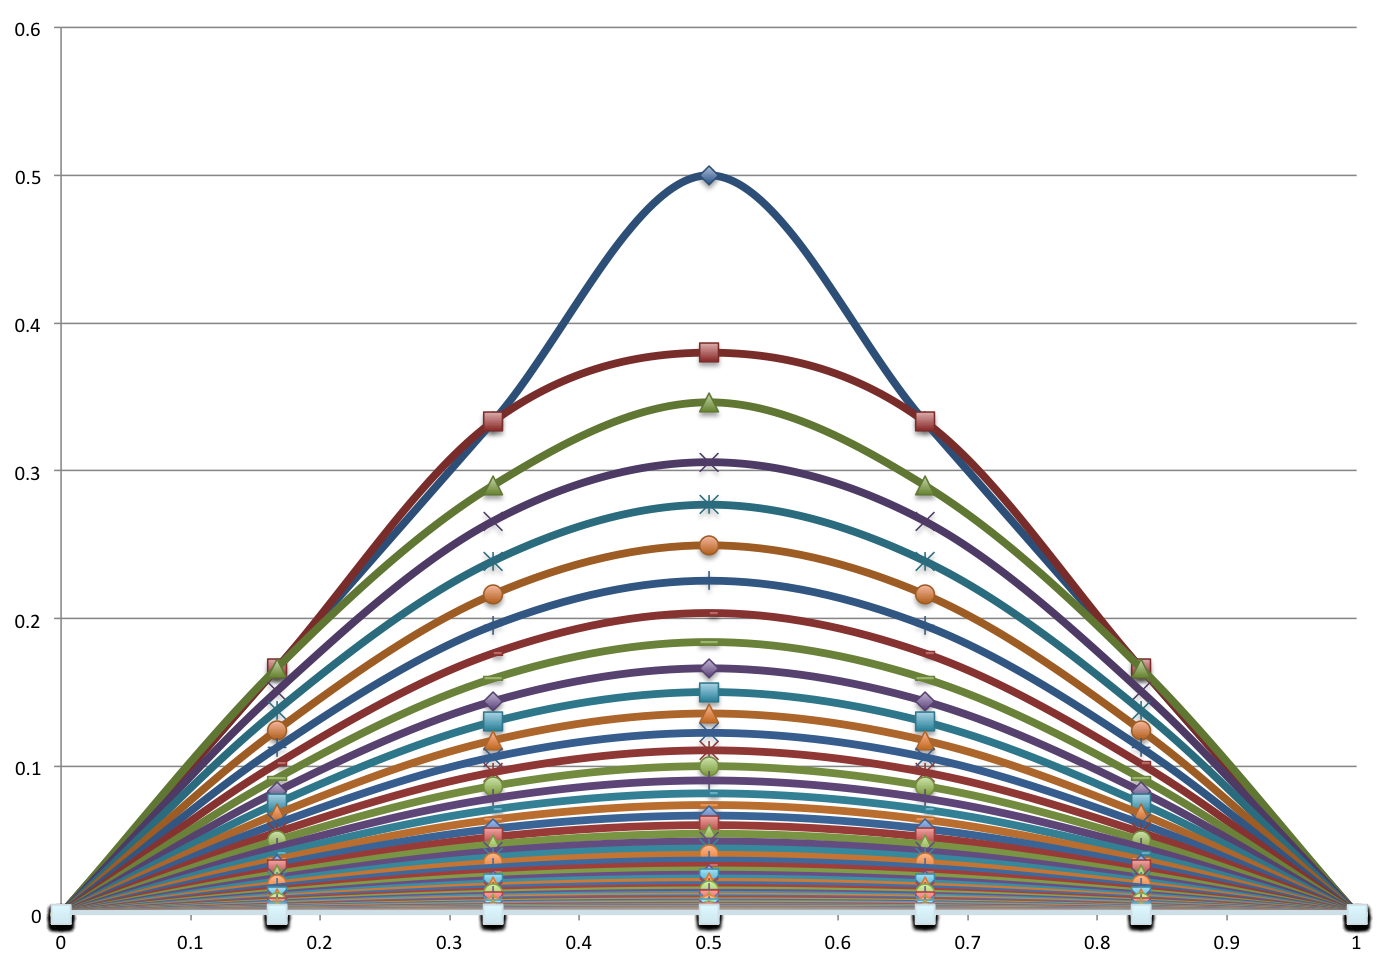
\includegraphics[width=120mm]{./img-kadai3/1-1-1-1.eps}
\caption{$(\Delta x, \Delta t) = (1/6, 1/100)$の場合の解}
\label{list:1-1-1-1}
\end{figure}

\begin{figure}[H]
\centering
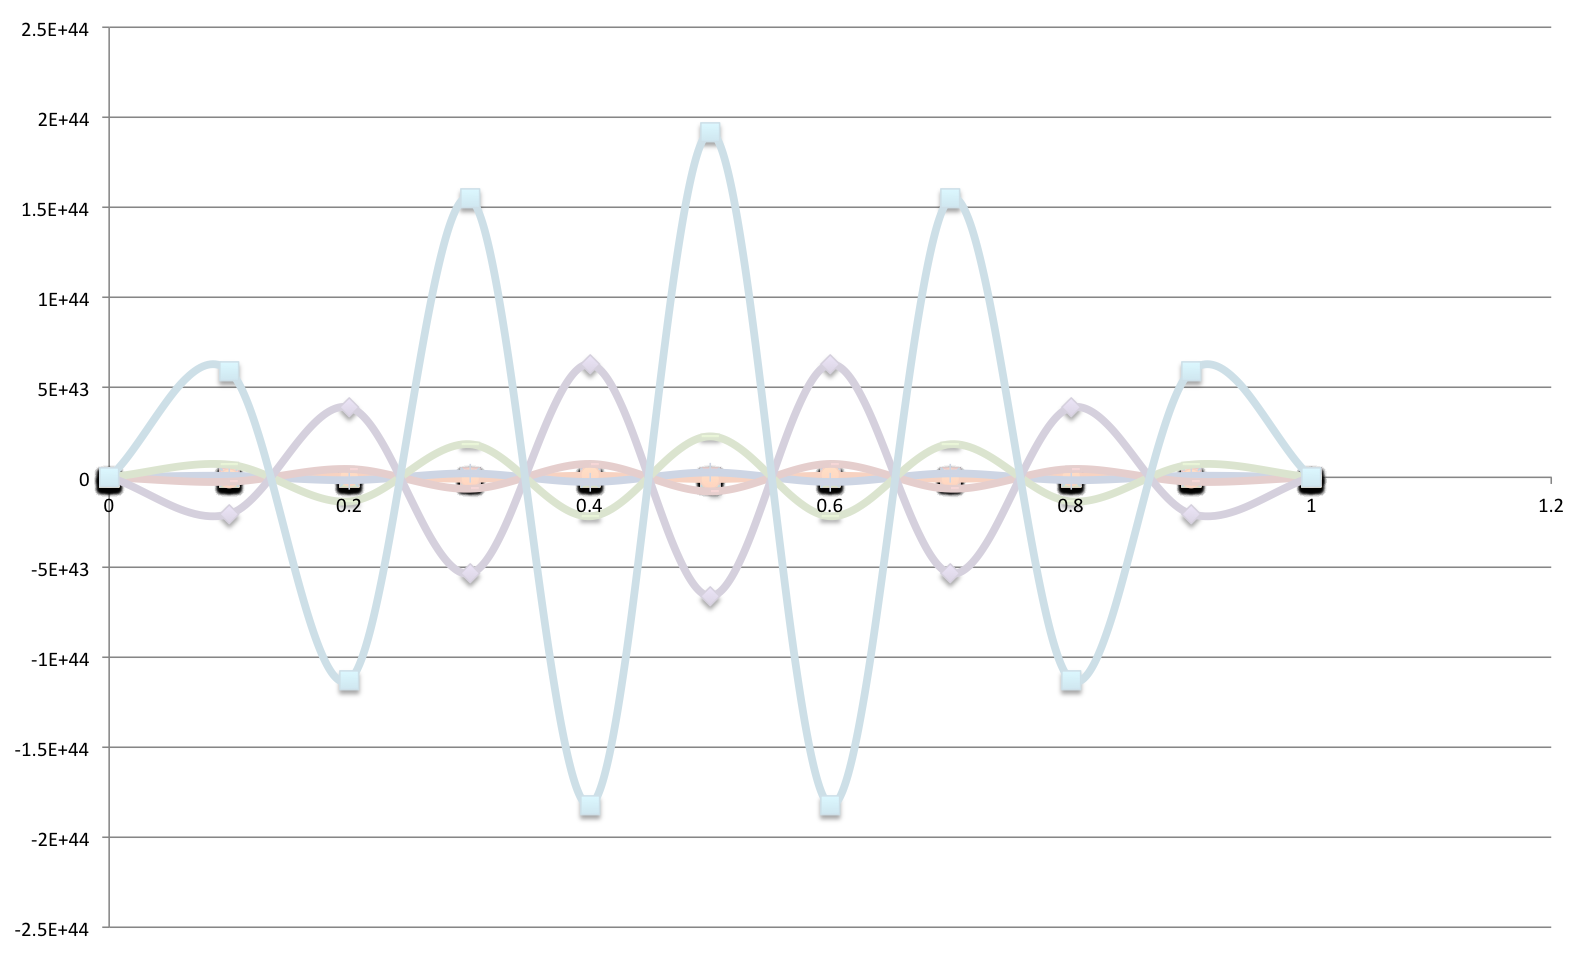
\includegraphics[width=120mm]{./img-kadai3/1-1-1-2.eps}
\caption{$(\Delta x, \Delta t) = (1/10, 1/100)$の場合の解}
\label{list:1-1-1-2}
\end{figure}

\begin{figure}[H]
\centering
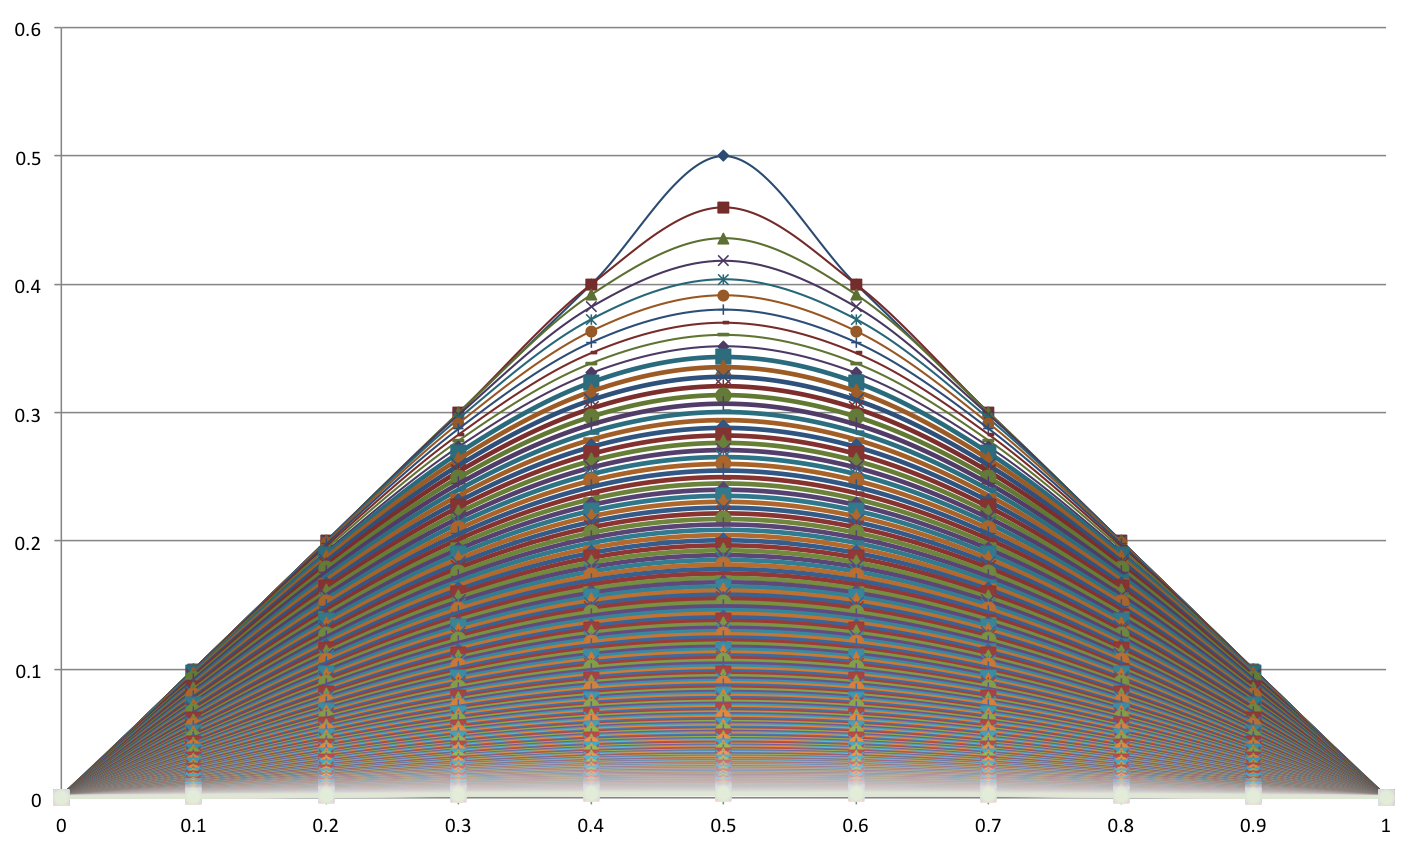
\includegraphics[width=120mm]{./img-kadai3/1-1-1-3.eps}
\caption{$(\Delta x, \Delta t) = (1/10, 1/500)$の場合の解}
\label{list:1-1-1-3}
\end{figure}


\subsubsection{$t=0.02, 0.04, 0.06, 0.08$での $x = 0.5$における$u$の値を答えよ。計算が不安定に成るのはどの場合か。}

各場合の$u$の値を以下に示す。
$(\Delta x, \Delta t) = (1/10, 1/100)$の時、$t=0.06$から$t=0.08$に変化するさい大きく$u$が変化することから最も計算が不安定になると考えられる。

\begin{table}[htbp]
\begin{center}
\caption{$t=0.02, 0.04, 0.06, 0.08$での $x = 0.5$における$u$の値}
\begin{tabular}{|c|c|c|c|} \hline
t & $(\Delta x, \Delta t) = (1/6, 1/100)$ & $(\Delta x, \Delta t) = (1/10, 1/100)$ & $(\Delta x, \Delta t) = (1/10, 1/500)$ \\ \hline
0.02 & 0.3464 & 0.50 & 0.392 \\ \hline
0.04 & 0.2771 & 1.30 & 0.373 \\ \hline
0.06 & 0.2257 & 7.70 & 0.355 \\ \hline
0.08 & 0.1842 & 58.1 & 0.339 \\ \hline
\end{tabular}
\label{tab:u-value}
\end{center}
\end{table}


\end{document}